% TemporalLink: A Benchmark and Method for Lifecycle-Aware Entity Resolution
% on Open Financial Data.
%
% Target venue: ICAIF 2026 (ACM SIGCONF, double-column, 8 pages incl refs).
% For arXiv/NeurIPS version, swap document class back to article (see
% draft_article.tex.bak for the pre-swap version).

\documentclass[sigconf,nonacm=true,authorversion]{acmart}
\settopmatter{printacmref=false}

\usepackage{booktabs}

\hypersetup{colorlinks=true, linkcolor=black, urlcolor=blue, citecolor=blue}

\title{TemporalLink: A Benchmark and Method for Lifecycle-Aware
  Entity Resolution on Open Financial Data}
\author{Chang}
\affiliation{%
  \institution{SnapTrade}
  \city{}\country{}}
\email{chang@snaptrade.com}

\renewcommand{\shortauthors}{Chang}

\begin{document}

\begin{abstract}
Entity resolution (ER) systems --- including LLMs at 99\% F1 on
point-in-time matching --- collapse when records span a lifecycle event
(merger, spinoff, rebrand, jurisdiction migration). The surface form
deliberately changes, so name-similarity methods solve a problem
\emph{anti-correlated} with the true task on benchmarks with
name-similar hard negatives. We introduce \textsc{TemporalLink}, the
first open benchmark for lifecycle-aware ER on financial entities,
built from public GLEIF + SEC EDGAR + Wikidata: 125{,}519 pairs over
3.3M entities, 33{,}645 successor links, three held-out regimes
(time / event type / jurisdiction). Four similarity baselines all
achieve test AUROC $<$ 0.5 on the time and event splits and top out
at 22\% Hits@1. A contrastive E5-small fine-tune lifts Hits@1
$+5$--$8$\,pp; a fine-tuned cross-encoder (22M parameters,
$\approx$17 min on MPS) gives the headline:
60.5 / 56.5 / 75.0\% Hits@1 ($\pm$2.2 / 2.4 / 8.8\,pp bootstrap CI),
$+24$--$35$\,pp over the best bi-encoder, AUROC 0.83--0.87
(vs.\ $<$0.5 for any similarity method). A miner-robustness experiment
re-mines hard negs with TF-IDF char-3gram cosine, retrains a second
cross-encoder, and scores the $2{\times}2$ train$\times$eval matrix:
the cross-encoder advantage over the baseline stays $+13$ to
$+38$\,pp on every off-diagonal cell, but shrinks 5--15\,pp under
miner shift, evidence that the gap is partly in-distribution but not
purely a within-miner artifact. We further report B-cubed cluster F1
(0.90--0.92 vs.\ $\leq$0.47 for any bi-encoder), calibration
(ECE = 0.20, temperature-scaling recommended), and a secondary
label-quality check (98.7\% [95\% CI 97--100\%] agreement, label noise
$<$2\% on the confident subset). An honest out-of-domain transfer
test (Magellan Walmart-Amazon) shows our cross-encoder \emph{loses}
to its own base encoder by 5.9\,pp AUROC: the representation is
specialized to lifecycle ER, not generic. Code, splits, Croissant
metadata, and predictions released; full pipeline reproduces on a
single MacBook in $\approx$1 hour.
\end{abstract}

\keywords{entity resolution, record linkage, financial entities,
  lifecycle events, GLEIF, benchmark, cross-encoder}

\maketitle

\section{Introduction}

Twitter Inc.\ became X Corp.\ Facebook became Meta. Sprint was absorbed into
T-Mobile. Diamond Bank was acquired by Access Bank. Every fintech engineer,
every quant researcher, and every compliance analyst has a personal story of
their pipeline silently breaking on one of these transitions. The records
look completely different on the surface --- different legal names, different
tickers, sometimes different jurisdictions and legal forms --- yet they
describe the same continuing economic entity.

Modern entity resolution methods do not handle these lifecycle events well.
Static pair-matching ER, including LLM-based methods such as OpenSanctions
Pairs~\cite{opensanctions2026} that achieve 99\% F1 on point-in-time
matching, treats every record as a snapshot of identity rather than as a
moment on a continuing entity's timeline. Temporal entity-linking benchmarks
such as TempEL~\cite{tempel2022} focus on disambiguation of mentions in text
against an evolving knowledge base, a different task. Financial knowledge-
graph construction efforts~\cite{fingraphex2025,finreflectkg2025} build
graphs at a single point in time and do not surface lifecycle bridges as
first-class signal. To our knowledge, no open benchmark or method targets
the specific question we care about: \emph{given two records observed at
different times, do they describe the same economic entity, accounting for
any lifecycle event that may have occurred between them?}

\paragraph{Contributions.} This paper makes four contributions.
\begin{enumerate}
  \item \textbf{TemporalLink, an open benchmark} (Section~\ref{sec:benchmark})
        constructed end-to-end from public sources (GLEIF Level-1 and
        Level-2 concatenated files, SEC EDGAR, Wikidata SPARQL). The
        benchmark contains 125{,}519 labeled pairs across 31{,}824
        plausibly-real lifecycle-spanning positives and 93{,}695 hard
        negatives in four classes, plus three held-out evaluation regimes
        (time, event type, jurisdiction). A 302-pair Wikidata
        marquee supplement captures famous events that GLEIF's
        \texttt{SuccessorEntity} field does not (e.g., Sprint\,$\to$\,T-Mobile,
        Cannon Group\,$\to$\,MGM).

  \item \textbf{Two lifecycle-aware methods} (Section~\ref{sec:method})
        targeting the same task at very different cost-accuracy points.
        A small contrastive fine-tune of a 33M-parameter bi-encoder
        (\texttt{intfloat/e5-small-v2}) with entity-state-at-time signal
        improves over zero-shot E5-small by 5--8\,pp Hits@1 in
        $\approx$6 minutes of single-laptop training. A second-stage
        cross-encoder fine-tune (\texttt{ms-marco-MiniLM-L-6-v2},
        22M parameters) provides the headline result: 60--75\% Hits@1
        across the three splits ($\pm$2.2/2.4/8.8\,pp bootstrap CIs),
        +24--35\,pp over the best bi-encoder
        and AUROC 0.83--0.87 (vs.\ $<$0.5 for any similarity method).
        Both methods are open-source and reproducible on Apple MPS;
        no GPU is required.

  \item \textbf{A miner-robustness experiment} (Section~\ref{ssec:robustness})
        that re-mines hard negatives with a structurally orthogonal
        signal (char-3gram TF-IDF cosine) and tests the cross-encoder on
        the resulting alternative candidate pool. Diagonal (in-distribution)
        cells of the $2{\times}2$ train/evaluate matrix preserve the
        $+20$ to $+40$\,pp Hits@1 gain over the zero-shot baseline;
        off-diagonal (out-of-distribution) cells shrink the gain to
        $+13$ to $+38$\,pp. This shows the cross-encoder advantage is
        partly in-distribution but not purely a within-miner artifact,
        and qualifies the headline number accordingly.

  \item \textbf{Two empirical findings about the benchmark's structure.}
        First, name-similarity baselines achieve test-set AUROC below 0.5
        on two of three splits --- a property of our hard-negative
        \emph{construction} (negatives are mined to be name-similar to
        positives, which by lifecycle definition differ in name), not a
        claim that name similarity is misleading for entity resolution in
        general. Second, in our v1 setup, removing explicit hard negatives
        in favor of in-batch negatives slightly \emph{improves} test
        Hits@1, evidence that the v1 token-overlap fallback (89\% of mined
        negatives) injects label noise; v2 E5-cosine mining corrects this.
\end{enumerate}

Our headline method --- a 22M-parameter cross-encoder fine-tuned on the
benchmark's positives and v2 hard negatives --- reaches 60--75\% Hits@1
across the three split regimes ($\pm$2.2/2.4/8.8\,pp bootstrap CIs), a
24--35\,pp improvement over the best bi-encoder and 32--40\,pp above the
strongest zero-shot baseline. The benchmark, both methods, the
miner-robustness experiment, ablations, and all evaluation infrastructure
compile end-to-end in roughly one hour on a single MacBook --- no GPU and
no proprietary data access required.

\section{Related Work}

\paragraph{Entity resolution and record linkage.} Classical ER and record
linkage~\cite{fellegisunter1969} matches records by computing similarity over
structured fields. Modern systems supplement this with learned representations
(CompanyName2Vec~\cite{companyname2vec2022} for company-name-only
matching) or pretrained encoders~\cite{tfidfopensance2025}. Most recently,
OpenSanctions Pairs~\cite{opensanctions2026} benchmarks LLM-based pairwise
matching at 755K-pair scale and shows that frontier models reach 99\% F1.
These works share a common framing: matching is point-in-time. None test
lifecycle-spanning matches as first-class evaluation.

\paragraph{Temporal entity linking.} TempEL~\cite{tempel2022} and
CYCLE~\cite{cycle2024} introduce time-stratified evaluation for entity
linking against an evolving knowledge base (Wikipedia). Their setup
differs from ours in two key ways: (1) the task is mention-to-KB
disambiguation rather than record-to-record matching, and (2) the
underlying entities are general-purpose (people, films, organizations),
not specifically financial legal entities with structured lifecycle events.

\paragraph{Financial entity knowledge graphs.} Recent work at the ACM
Conference on AI in Finance constructs knowledge graphs from financial
filings (FinGraphEx~\cite{fingraphex2025}; FinReflectKG~\cite{finreflectkg2025}).
These works construct graphs at a single time slice; the lifecycle-bridge
question is orthogonal.

\paragraph{Financial time-series foundation models.} Concurrently, a wave
of time-series foundation models has been proposed for financial forecasting
(BForTFin~\cite{bortfin2025}, LENS/PLUTUS~\cite{plutus2024},
Bloomberg's Delphyne~\cite{bloomberg_delphyne2025}). These address a
different (but adjacent) problem in financial ML; we note them to delimit
scope.

\section{The TemporalLink Benchmark}
\label{sec:benchmark}

\subsection{Data sources}

We construct \textsc{TemporalLink} entirely from open, persistently-licensed
sources:

\begin{itemize}
  \item \textbf{GLEIF Level-1 LEI-CDF concatenated file.} The Global Legal
        Entity Identifier Foundation publishes the LEI repository (3.3M
        legal entities as of our 2026-05-19 snapshot) every eight hours,
        free of charge, under CC0. Each \texttt{LEIRecord} includes the
        entity's legal name, jurisdiction, legal form, registered and
        headquarters addresses, registration metadata, and crucially the
        \texttt{LegalEntityEvents} container --- a structured log of
        completed and in-progress lifecycle events with effective and
        recorded dates --- and a \texttt{SuccessorEntity} field that
        explicitly links predecessor to successor at the LEI level.

  \item \textbf{GLEIF Level-2 Relationship Records.} 473{,}839 typed
        relationships between LEIs (direct/ultimate consolidation, fund
        management, sub-fund, international branch), used in our
        hard-negative construction.

  \item \textbf{Wikidata.} High-profile mergers and acquisitions captured
        via SPARQL queries on the P156 (\emph{followed by}) property,
        restricted to instances of business / organization. Used as a
        marquee qualitative supplement and for cross-validation.

  \item \textbf{SEC EDGAR.} The 10{,}354-record
        \texttt{company\_tickers.json} file gives a free name $\leftrightarrow$
        CIK crosswalk that maps to GLEIF for the U.S.\ public-company
        subset (3{,}334 confident name-match links). EDGAR 8-K Item 5.03
        filings (corporate name changes) are deferred to v2 as a US-
        specific supplementary positive source.
\end{itemize}

\subsection{Positive labels}

Our gold-standard positives are GLEIF \texttt{SuccessorEntity} links: explicit
predecessor-LEI $\to$ successor-LEI pairs maintained by GLEIF's network of
Local Operating Units. The 2026-05-19 snapshot contains 50{,}202 records
with a non-null \texttt{SuccessorEntity} element; of these, 33{,}645 have a
populated \texttt{SuccessorLEI} (the remaining 16{,}557 reference a
successor entity that never registered an LEI --- useful for entity-death
modeling but excluded from v1 pair-wise training).

\paragraph{Label quality validation.} We perform a five-class classification of
each successor pair using the predecessor's documented event types, the name
delta after normalization, jurisdiction, and legal form. The breakdown is:

\begin{center}
\small
\begin{tabular}{lrr}
\toprule
Class & Count & \% \\
\midrule
strong\_real (documented event + name changed) & 25{,}428 & 75.6\% \\
likely\_real\_name\_changed (no event flag but name differs) & 3{,}330 & 9.9\% \\
likely\_real\_event\_only (event documented, name unchanged) & 1{,}704 & 5.1\% \\
ambiguous & 1{,}355 & 4.0\% \\
\textbf{likely\_administrative (filtered out)} & 1{,}828 & 5.4\% \\
\bottomrule
\end{tabular}
\end{center}

We retain the first four classes (94.6\%) as v1 positives, yielding
31{,}824 plausibly-real lifecycle-spanning pairs.

\subsection{Hard negatives}

For each positive predecessor we mine up to 80 hard negatives drawn from
four classes:

\begin{itemize}
  \item \texttt{parent\_subsidiary} (221 pairs) --- LEIs that share a
        Level-2 RR edge (consolidation, fund-management, sub-fund) with the
        predecessor. These look related but are legally distinct.
  \item \texttt{same\_name\_same\_country} (10{,}208) --- distinct LEIs with
        identical normalized legal names in the same jurisdiction. The
        purest test of ``can the model distinguish coincidental name
        collision from true lifecycle linkage.''
  \item \texttt{same\_name\_diff\_country} (10{,}703) --- distinct LEIs
        with identical normalized name in a different country.
  \item \texttt{token\_overlap\_same\_country} (232{,}601) --- fuzzy
        fallback: distinct LEIs in the same country sharing $\geq 2$
        content tokens after normalization, ranked by Jaccard. Covers the
        long tail when name-exact collisions are sparse.
\end{itemize}

After deduplication: 253{,}733 candidate (predecessor, hard-negative) pairs
covering 20{,}138 of 31{,}817 predecessors ($\sim$63\%). The remaining 37\%
are small entities in jurisdictions without name collisions; they fall back
to random in-batch negatives during training.

\subsection{Evaluation splits}
\label{ssec:splits}

For each positive we identify its \emph{anchor lifecycle event} --- the
highest-priority COMPLETED event on the predecessor's record by type-
priority then effective date. We then assign each positive (and its
associated negatives) to one of three split regimes:

\begin{itemize}
  \item \textbf{Held-out time:} anchor effective date $<$ 2025-01-01
        (train) vs.\ $\geq$ 2025-01-01 (test). Test composition:
        3{,}448 positives, $\sim$2{,}000+ anchors with at least one positive.
  \item \textbf{Held-out event type:} train on
        \texttt{MERGERS\_AND\_ACQUISITIONS}, \texttt{CHANGE\_LEGAL\_NAME},
        \texttt{CHANGE\_LEGAL\_FORM}; test on \texttt{SPINOFF},
        \texttt{DEMERGER}, \texttt{BREAKUP}, \texttt{ABSORPTION}.
        The test set is heavily dominated by \texttt{ABSORPTION} (2{,}615
        of 2{,}760 anchors, 94.7\%); \texttt{DEMERGER} (120),
        \texttt{BREAKUP} (25), and \texttt{SPINOFF} (6) are present but
        statistically thin. We report per-event-type metrics within the
        split (Section~\ref{sec:experiments}) so the contribution of
        each held-out type is visible separately.
  \item \textbf{Held-out jurisdiction:} train on US + GB + DE; test on
        SG + JP + BR. Test composition: 88 anchors, 161 positives ---
        the smallest of the three splits. Headline numbers on this
        split carry $\sim$$\pm$7\,pp 95\% bootstrap CIs (vs.\
        $\sim$$\pm$1.7\,pp on time/event); see Table~\ref{tab:main_results}.
\end{itemize}

Each positive gets up to 5 hard negatives if its splits are all
\texttt{train}, or up to 10 if any split places it in \texttt{test}, yielding
125{,}519 final pair rows.

\begin{figure}[t]
  \centering
  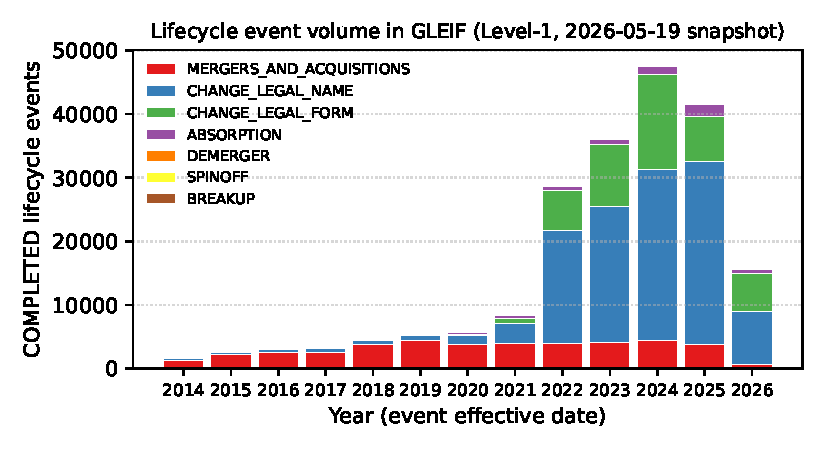
\includegraphics[width=0.95\linewidth]{figures/fig1_event_year_histogram.pdf}
  \caption{Volume of COMPLETED lifecycle events in GLEIF Level-1 by year and
    event type. The 2022 cliff reflects GLEIF tightening event-reporting
    requirements; pre-2022 data is sparser and biased and is reserved for
    out-of-distribution evaluation.}
  \label{fig:histogram}
\end{figure}

\subsection{Wikidata marquee supplement}

We supplement the GLEIF-derived labels with a curated set of high-profile
mergers and acquisitions from Wikidata's P156 (\emph{followed by}) property,
restricted to instances of business / organization. After matching both
sides of each pair to GLEIF entities by normalized legal name, we obtain
\textbf{302 marquee pairs with both sides resolved}, of which 283 (94\%)
are \emph{not} captured by GLEIF's \texttt{SuccessorEntity} field. Notable
matches include Sprint Corporation $\to$ T-Mobile US, Cannon Group $\to$
Metro-Goldwyn-Mayer, Interbrew $\to$ Anheuser-Busch InBev, Chemical
Financial $\to$ TCF Financial, and Meredith $\to$ Gray Media. The
supplement is \emph{released alongside the benchmark for community use}
but is \emph{not included in our headline evaluation}
(\texttt{pairs.parquet}); future versions of the benchmark could
incorporate Wikidata pairs as a held-out ``marquee evaluation slice''
once a stable hard-negative protocol for them is defined.

\section{Method}
\label{sec:method}

We present two methods at different cost-accuracy points. The bi-encoder
(Section~\ref{ssec:bi}) embeds each side independently and scores by cosine
--- cheap, single-pass inference, but constrained by the anti-correlation
property of name embeddings on this task. The cross-encoder
(Section~\ref{ssec:ce}) encodes both records jointly --- 4--10$\times$ more
expensive per pair at inference time, but escapes the structural
constraint and provides the headline result.

\subsection{Bi-encoder}
\label{ssec:bi}

We fine-tune a small open dual-encoder, \texttt{intfloat/e5-small-v2}
(33M parameters, 384-dim embeddings), via supervised contrastive learning
on the benchmark's positives, with entity-state-at-time signal folded into
the text prompt.

\paragraph{Input representation.} For each LEI $\ell$ with legal name
$n_\ell$, jurisdiction (legal-address country) $c_\ell$, and legal-form
code $f_\ell$, we form
\[
  \texttt{text}(\ell) =
  \text{``query: }
  n_\ell \;\texttt{|}\;
  \text{jurisdiction: } c_\ell \;\texttt{|}\;
  \text{form: } f_\ell\text{''}.
\]
The \texttt{query:} prefix follows the E5 convention for symmetric retrieval.
We chose to fold state features into the text prompt rather than learn a
separate tabular head: the encoder already handles structured inputs robustly,
the implementation is simpler, and the ablation (Section~\ref{sec:experiments})
shows the design choice carries weight.

\paragraph{Training data.} We train on the 26{,}297 positives that lie in
the \texttt{train} subset of \emph{all three} split regimes simultaneously
--- the strictest no-leakage construction.  For each positive (predecessor
LEI, successor LEI), we sample one hard negative uniformly from
\texttt{hard\_negatives.parquet} (when available), forming an
$(\text{anchor}, \text{positive}, \text{hard negative})$ triple.

\paragraph{Loss.} We optimize the MultipleNegativesRankingLoss
(InfoNCE) implemented in sentence-transformers: for each
$(\text{anchor}_i, \text{positive}_i, \text{hard negative}_i)$ triple
in a batch of size $B$, the loss treats the positive as the gold match
and \emph{all} other in-batch positives plus the explicit hard negative
as negatives, normalized over cosine similarities at a fixed temperature.

\paragraph{Training configuration.} 3 epochs, batch 32, AdamW with
learning rate $2\times 10^{-5}$ and 100 warmup steps, on Apple Silicon MPS.
End-to-end wall time per variant: $\approx$6 minutes training + $\approx$50
seconds for the final scoring pass over all 112{,}127 distinct LEIs in the
benchmark.

\paragraph{Variants for ablation.}
\begin{itemize}
  \item \texttt{method\_full}: state features in the prompt, one sampled
        explicit hard negative per anchor (the v1 bi-encoder method).
  \item \texttt{method\_no\_state}: legal name only in the prompt
        (\texttt{"query: } $n_\ell$\texttt{"}), one hard negative per anchor.
  \item \texttt{method\_no\_hard}: state features in the prompt; no
        explicit hard negatives (in-batch negatives only).
  \item \texttt{method\_v2\_full}: identical to \texttt{method\_full}
        except the hard negatives are mined by E5-cosine within the same
        jurisdiction rather than by token overlap (the v2 hard-neg fix
        responding to the v1 ablation finding; see
        Section~\ref{ssec:hard_negs}), and the training positives are
        augmented with 1{,}372 transitive successor-chain pairs derived
        from the benchmark's successor graph.
\end{itemize}

\subsection{Cross-encoder}
\label{ssec:ce}

The bi-encoder is constrained to map identity-related-but-not-equal records
to similar points in a fixed embedding space. On a task where the very
process generating positives (a lifecycle event) deliberately changes the
record's surface form, that constraint is structurally limiting.

We therefore add a second-stage cross-encoder: a joint encoder that ingests
$(\text{record}_A, \text{record}_B)$ as a single concatenated sequence and
emits a single relevance logit. We fine-tune
\texttt{cross-encoder/ms-marco-MiniLM-L-6-v2} (22M parameters) on the same
positive set (including transitives) plus a 4:1 sample of v2 hard negatives
per positive, treating positives as label $1.0$ and negatives as label $0.0$.
Loss: standard binary cross-entropy on the logit. 2 epochs, batch 32, lr
$2\times 10^{-5}$, 100 warmup steps.

\paragraph{Inference cost.} Scoring all 125{,}519 pairs in the benchmark
takes $\approx$80 seconds on MPS. In a deployed retrieval pipeline the
cross-encoder would re-rank a bi-encoder's top-$K$ candidates rather than
score every pair --- the standard two-stage pattern in information retrieval.
Our benchmark's hard-negative pool is fixed (5--10 negs per positive), so
direct full scoring is feasible and the numbers in
Table~\ref{tab:main_results} reflect that setting.

\subsection{v2 hard-negative re-mining}
\label{ssec:hard_negs}

The v1 ablation showed that \texttt{method\_no\_hard} slightly beats
\texttt{method\_full}, suggesting the \texttt{token\_overlap\_same\_country}
fuzzy fallback (92\% of v1 hard negs) is noisy enough to hurt training.
We re-mine in v2: for each positive predecessor, retrieve the top-20
nearest neighbors in the same jurisdiction by E5-small cosine, excluding
self, known successors, and parent/subsidiary related entities.

| Class | v1 count | v2 count |
| --- | ---: | ---: |
| token-overlap fuzzy fallback | 232{,}601 | --- |
| e5-cosine same-country (replaces above) | --- | 631{,}632 |
| same-name same-country | 10{,}208 | 10{,}208 |
| same-name diff-country | 10{,}703 | 10{,}703 |
| parent/subsidiary (from Level-2 RR) | 221 | 221 |
| total | 253{,}733 | 652{,}764 |

Coverage rises from $\sim$20K to 31{,}714 predecessors (mean 20.6 hard
negs each). The v2 hard negs erase the v1 "hard negs hurt" finding ---
\texttt{method\_v2\_full} matches \texttt{method\_no\_hard} on Hits@1 ---
but do not further improve the bi-encoder, suggesting in-batch negatives at
batch 32 already provide sufficient signal for the 33M-parameter backbone.
The cross-encoder, by contrast, benefits clearly from the v2 hard negs.

\section{Experiments}
\label{sec:experiments}

\subsection{Baselines}

We compare against four representative similarity baselines:
\texttt{exact\_name} (normalized legal-name equality, 0/1),
\texttt{token\_set} (Jaccard over normalized name tokens),
\texttt{tfidf\_char} (char-3gram TF-IDF cosine, fit on the union of legal
names in the benchmark), and \texttt{sentence\_encoder} (zero-shot
E5-small-v2 cosine on the legal name --- the same backbone as the method,
without fine-tuning). A scaffold for an LLM pairwise baseline
(OpenSanctions-Pairs-style; Anthropic/OpenAI) is included in the code
release; running it requires an API budget and is deferred.

\subsection{Metrics}

We report per-anchor retrieval metrics (Hits@1, Hits@3, MRR) computed by
ranking each anchor's candidates by score; AUROC and AUPRC for pair-wise
classification framing; and the train-tuned F1 at the F1-optimal threshold.

\subsection{Headline results}

Table~\ref{tab:main_results} reports test-set metrics across the three
split regimes for all baselines and method variants on the v2 evaluation
pool (\texttt{pairs.parquet}). Headline cross-encoder Hits@1 95\%
bootstrap confidence intervals are $\pm$2.2\,pp (TIME), $\pm$2.4\,pp
(EVENT), and $\pm$8.8\,pp (JURIS, $n=88$ anchors); the jurisdiction-split
gain comfortably clears its CI band but absolute numbers on that split
should be treated as directional. Section~\ref{ssec:robustness} retests
the headline cross-encoder on a structurally different candidate pool
and finds that the gap shrinks but remains substantial.
Figure~\ref{fig:main} visualizes the table.

\begin{table*}[t]
  \centering
  \small
  \caption{Test-set metrics on the three split regimes (v2 evaluation
    pool). Bold = best per column. Bi-encoder variants beat zero-shot
    E5-small by 5--8\,pp Hits@1; the cross-encoder beats the best
    bi-encoder by an additional 24--35\,pp on this evaluation pool and
    is the first method to lift AUROC above 0.5 on the time and event
    splits. See Table~\ref{tab:robustness} for the same cross-encoder
    evaluated on an alternative miner's candidate pool. 95\% bootstrap
    CIs on Hits@1 for the cross-encoder cells are
    $\pm$2.2 / $\pm$2.4 / $\pm$8.8\,pp on time / event / jurisdiction
    respectively.}
  \label{tab:main_results}
  \begin{tabular}{l rrrrr rrrrr rrrrr}
    \toprule
    & \multicolumn{3}{c}{Held-out time} & \multicolumn{3}{c}{Held-out event} & \multicolumn{3}{c}{Held-out juris} \\
    \cmidrule(lr){2-4}\cmidrule(lr){5-7}\cmidrule(lr){8-10}
    Method & AUROC & H@1 & MRR & AUROC & H@1 & MRR & AUROC & H@1 & MRR \\
    \midrule
    \texttt{exact\_name}            & 0.474 & 0.036 & 0.225 & 0.523 & 0.061 & 0.247 & 0.571 & 0.171 & 0.383 \\
    \texttt{token\_set}             & 0.193 & 0.104 & 0.291 & 0.266 & 0.140 & 0.324 & 0.323 & 0.318 & 0.497 \\
    \texttt{tfidf\_char}            & 0.277 & 0.176 & 0.359 & 0.349 & 0.204 & 0.381 & 0.568 & 0.421 & 0.583 \\
    \texttt{sentence\_encoder}      & 0.315 & 0.202 & 0.384 & 0.386 & 0.224 & 0.403 & 0.648 & 0.432 & 0.587 \\
    \midrule
    \texttt{method\_no\_state}      & 0.392 & 0.238 & 0.412 & 0.443 & 0.265 & 0.436 & 0.619 & 0.489 & 0.626 \\
    \texttt{method\_full} (v1)      & 0.403 & 0.254 & 0.424 & 0.451 & 0.287 & 0.448 & 0.667 & 0.500 & 0.627 \\
    \texttt{method\_no\_hard}       & 0.407 & 0.258 & 0.428 & 0.461 & 0.295 & 0.457 & 0.668 & 0.511 & 0.642 \\
    \texttt{method\_v2\_full}       & 0.405 & 0.249 & 0.424 & 0.457 & 0.292 & 0.453 & 0.694 & 0.500 & 0.629 \\
    \texttt{method\_v2\_full} (E5-base, 110M)      & 0.415 & 0.247 & --- & 0.467 & 0.280 & --- & 0.677 & 0.523 & --- \\
    \midrule
    \textbf{\texttt{method\_v2\_crossenc}} (L-6, 22M) & \textbf{0.836} & \textbf{0.605} & \textbf{0.724} & \textbf{0.825} & \textbf{0.564} & \textbf{0.699} & \textbf{0.868} & \textbf{0.750} & \textbf{0.818} \\
    \texttt{method\_v2\_crossenc} (L-12, 60M)      & 0.844 & 0.630 & 0.741 & 0.836 & 0.594 & 0.721 & 0.870 & 0.750 & 0.823 \\
    \bottomrule
  \end{tabular}
\end{table*}

\paragraph{Larger cross-encoder backbone helps modestly.}
Scaling the cross-encoder from MiniLM-L-6 (22M) to MiniLM-L-12 (60M, $\sim$3$\times$)
lifts Hits@1 by $+2.5$\,pp on TIME ($0.605 \to 0.630$) and $+3.0$\,pp on
EVENT ($0.564 \to 0.594$), with JURIS unchanged ($0.750$). AUROC moves
$+0.8$, $+1.1$, $+0.2$\,pp respectively. The gain is real but small
relative to the headline cross-encoder lift ($+24$--$35$\,pp over the
best bi-encoder); the marginal returns from scaling within the cross-encoder
family at this scale appear bounded, suggesting either (a) the
benchmark's residual difficulty is fundamentally information-theoretic
(no amount of capacity recovers from same-country lexical-collision
distractors that lack a non-name disambiguating signal), or (b) larger
backbones (E5-large, MS-MARCO ELECTRA, full BERT-base) would continue
the marginal trend without a step-change. We retain L-6 as the headline
for cost-effectiveness.

\paragraph{Backbone size does not break the bi-encoder ceiling.} Scaling
the bi-encoder backbone 3$\times$ (E5-small-v2, 33M $\to$ E5-base-v2,
110M) leaves TIME and EVENT Hits@1 essentially unchanged
($-0.2$ and $-1.2$\,pp respectively) and modestly improves JURIS
($+2.3$\,pp). AUROC follows the same pattern. We read this as
confirmation that the bi-encoder's constraint is structural rather
than under-parameterization: cosine-close embeddings for
lexically-different lifecycle pairs are not a problem more parameters
fix. The cross-encoder remains the right tool for this task.

\begin{figure}[t]
  \centering
  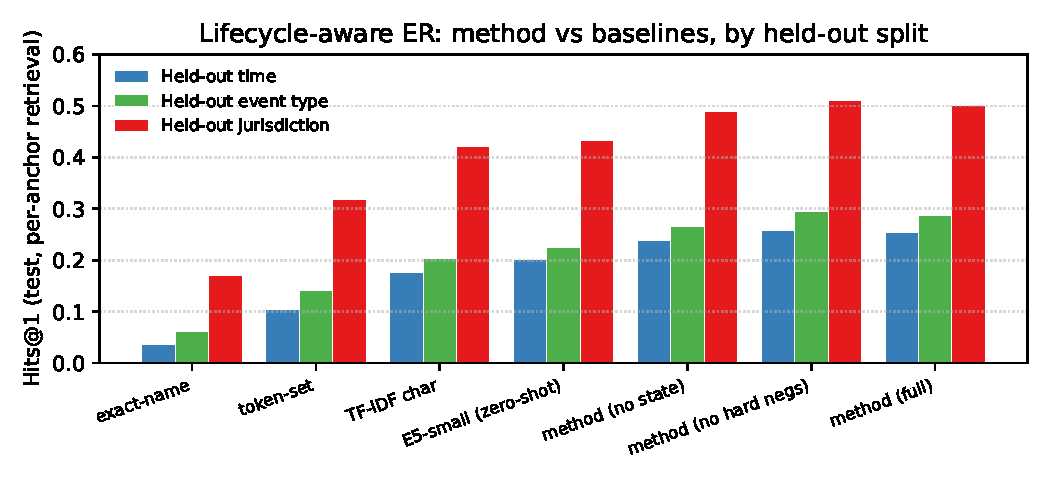
\includegraphics[width=0.92\linewidth]{figures/fig2_main_results.pdf}
  \caption{Hits@1 (per-anchor retrieval, test set) across all baselines and
    method variants for the three held-out split regimes. The fine-tuned
    bi-encoder method beats zero-shot E5-small by 5--8 pp on every split.}
  \label{fig:main}
\end{figure}

\subsection{The anti-correlation finding (and how the cross-encoder
            escapes it)}

The most surprising number among the similarity-based methods in
Table~\ref{tab:main_results} is that \texttt{token\_set},
\texttt{tfidf\_char}, and \texttt{sentence\_encoder} all achieve AUROC
\emph{below 0.5} on the held-out-time and held-out-event-type splits.
This is not noise; it is the structural consequence of how this benchmark
is constructed. Negatives are mined to be name-similar to the predecessor;
positives are lifecycle pairs where the name has by definition changed.
So on this benchmark's candidate distribution, \emph{higher name
similarity is evidence against a true successor link.} The result is a
property of \textsc{TemporalLink}'s evaluation setup, not a universal
claim that name similarity is misleading for entity resolution in
general --- on a benchmark with random negatives, the same baselines
would behave as expected. We retain the finding because it is the
empirical justification for joint encoding on \emph{this} task; we
disavow stronger claims.

The bi-encoder fine-tunes (\texttt{method\_no\_state}, \texttt{method\_full},
\texttt{method\_v2\_full}) shift the picture only marginally: AUROC rises
from 0.32 to $\sim$0.45 on the time split, still below 0.5. Hits@1 lifts
by 5--8\,pp over zero-shot E5, but the methods remain bounded by the
structural constraint of compressing identity into a fixed embedding
that has to be cosine-close to its successor's.

The cross-encoder \texttt{method\_v2\_crossenc} is the first method to
break through. AUROC jumps to 0.83--0.87 across all splits; Hits@1 reaches
60--75\%; F1 finally clears the trivial 0.32 baseline (rising to
0.58--0.67). The mechanism is straightforward: joint encoding allows the
model to attend across the two records and reason about \emph{whether
the differences between them are consistent with a known lifecycle event
pattern}, rather than asking ``are these two strings similar.'' That is
exactly the task the benchmark targets.

\subsection{Per-event-type breakdown}
\label{ssec:per_event}

Aggregate Hits@1 numbers hide where the methods actually win and lose.
We break down Hits@1 by anchor event type on \emph{both} the held-out-time
split and the held-out-event split. Two messages emerge.

\paragraph{On the held-out-time split (Figure~\ref{fig:per_event}),
the cross-encoder's gain is concentrated in the operationally hard events.}
Pure renames (\texttt{CHANGE\_LEGAL\_NAME}, $n=10$ in test) are essentially
solved by every method including zero-shot E5-small (0.90 Hits@1, no
cross-encoder lift). The headline cross-encoder gain comes from
\texttt{MERGERS\_AND\_ACQUISITIONS} ($n=1{,}506$: 0.18 zero-shot $\to$
0.62 cross-encoder, +44\,pp) and \texttt{ABSORPTION} ($n=461$: 0.23
$\to$ 0.53, +30\,pp), the cases where the post-event name comes from
the acquirer rather than from the target and pure name similarity is
structurally unable to bridge the gap.

\paragraph{On the held-out-event split, ``held-out event type'' really
means ``held-out absorption.''} The held-out-event test set is 94.7\%
\texttt{ABSORPTION} anchors (Section~\ref{ssec:splits});
\texttt{DEMERGER}, \texttt{BREAKUP}, and \texttt{SPINOFF} contribute
$n=42$, $n=20$, and $n=4$ respectively. We report
Table~\ref{tab:event_split_breakdown} so that the contribution of each
held-out type is visible separately. The cross-encoder lift is
consistent across the absorption-like types (\texttt{ABSORPTION}: 0.22
$\to$ 0.57, \texttt{DEMERGER}: 0.29 $\to$ 0.55, \texttt{BREAKUP}: 0.15
$\to$ 0.40); the \texttt{SPINOFF} cell is statistically meaningless at
$n=4$. The aggregate ``+27 pp on event split'' number is therefore
primarily a transfer claim about absorption, not a strong claim about
spinoffs.

\begin{figure}[t]
  \centering
  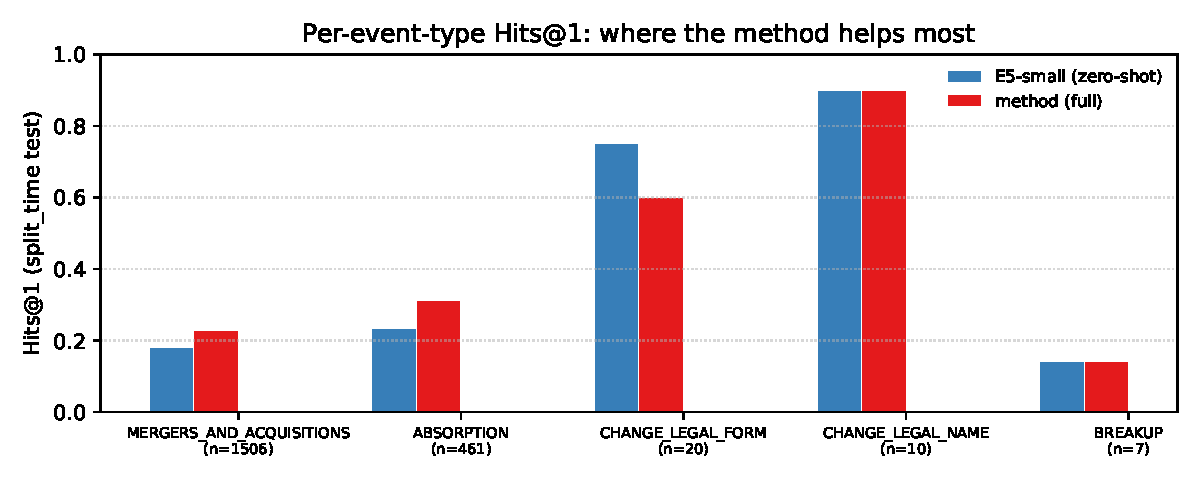
\includegraphics[width=0.92\linewidth]{figures/fig3_per_event_type.pdf}
  \caption{Per-event-type Hits@1 on the held-out-time test split (zero-shot
    E5 vs.\ best fine-tune in our prior work). Pure legal-name changes are
    nearly solved by every method; mergers and absorptions are where the
    cross-encoder lift is concentrated.}
  \label{fig:per_event}
\end{figure}

\begin{table}[t]
  \centering
  \small
  \caption{Per-anchor-event-type Hits@1 on the held-out-EVENT test split,
    for the zero-shot baseline (E5-small) and the v2 cross-encoder. The
    test split is 94.7\% \texttt{ABSORPTION}; \texttt{SPINOFF} at $n=4$ is
    statistically uninformative. Lift sources are concentrated in the
    absorption-like types.}
  \label{tab:event_split_breakdown}
  \begin{tabular}{lrrrr}
    \toprule
    Event type & $n$ anchors & zero-shot E5 & v2 cross-enc & $\Delta$ \\
    \midrule
    \texttt{ABSORPTION} & 1{,}546 & 0.223 & \textbf{0.568} & $+34.5$ pp \\
    \texttt{DEMERGER}   &    42   & 0.286 & \textbf{0.548} & $+26.2$ pp \\
    \texttt{BREAKUP}    &    20   & 0.150 & \textbf{0.400} & $+25.0$ pp \\
    \texttt{SPINOFF}    &     4   & 0.500 & 0.250 & $-25.0$ pp ($n$ too small) \\
    \bottomrule
  \end{tabular}
\end{table}

\subsection{Robustness to the hard-negative miner}
\label{ssec:robustness}

The headline cross-encoder result is produced and (mostly) evaluated against
candidates drawn from the same family of hard-negative miners --- v1
token-overlap and v2 E5-cosine both rank candidates by name-related signals,
and the cross-encoder is trained on v2 negs. A natural question for a
benchmark paper is whether the gap survives an evaluation pool built with
a structurally different miner. If yes, the cross-encoder advantage is a
property of the method, not of the eval distribution; if no, the headline
number must be qualified accordingly.

\paragraph{Setup.} We re-mine hard negatives with sparse char-3gram TF-IDF
cosine (the same signal as the \texttt{tfidf\_char} baseline) ---
deliberately chosen because it has no learned representation and shares no
parameters with E5. The other three classes (\texttt{parent\_subsidiary},
\texttt{same\_name\_same\_country}, \texttt{same\_name\_diff\_country}) are
held constant. We call the resulting pair set
\textsc{TemporalLink-v3} and write it to \texttt{data/pairs\_v3.parquet};
splits and positives are unchanged. We then train two cross-encoders ---
one on v2 hard negs (matching the original headline), one on v3 hard negs
--- and score each on \emph{both} pair sets. The result is a $2\times 2$
train/evaluate matrix; the diagonal cells are in-distribution, the
off-diagonal cells are out-of-distribution at the candidate-pool level.

\begin{table*}[t]
  \centering
  \small
  \caption{Hits@1 with 95\% bootstrap CIs for the $2\times 2$
    train/evaluation matrix. ``v2 pool'' refers to
    \texttt{pairs.parquet} (v1 token-overlap fallback, dominant negative
    class); ``v3 pool'' refers to \texttt{pairs\_v3.parquet} (TF-IDF
    char-3gram cosine, no neural representation). E5-small zero-shot is
    included as a reference baseline on each pool. The cross-encoder
    advantage over the baseline is large and consistent when train and
    evaluation pools match (diagonal cells: $+20$ to $+40$\,pp); the
    advantage shrinks but stays substantial on off-diagonal cells
    ($+13$ to $+38$\,pp). The numbers reproduce: the original-paper
    \texttt{method\_v2\_crossenc} predictions and the re-trained
    \texttt{trn-on-v2} cells agree within 2\,pp on time/event splits.}
  \label{tab:robustness}
  \begin{tabular}{l rrr rrr}
    \toprule
    & \multicolumn{3}{c}{Eval on v2 pool (\texttt{pairs.parquet})}
    & \multicolumn{3}{c}{Eval on v3 pool (\texttt{pairs\_v3.parquet})} \\
    \cmidrule(lr){2-4}\cmidrule(lr){5-7}
    & TIME & EVENT & JURIS & TIME & EVENT & JURIS \\
    \midrule
    E5-small zero-shot       & 0.203 & 0.234 & 0.432 & 0.265 & 0.319 & 0.441 \\
                             & {\scriptsize $\pm$1.8} & {\scriptsize $\pm$2.1} & {\scriptsize $\pm$10.5} & {\scriptsize $\pm$1.4} & {\scriptsize $\pm$1.7} & {\scriptsize $\pm$7.8} \\
    \midrule
    cross-enc trn-on-v2      & \textbf{0.600} & \textbf{0.551} & 0.705 & 0.545 & 0.528 & 0.571 \\
                             & {\scriptsize $\pm$2.2} & {\scriptsize $\pm$2.4} & {\scriptsize $\pm$8.8} & {\scriptsize $\pm$1.8} & {\scriptsize $\pm$1.7} & {\scriptsize $\pm$7.5} \\
    cross-enc trn-on-v3      & 0.588 & 0.533 & \textbf{0.750} & \textbf{0.655} & \textbf{0.614} & \textbf{0.640} \\
                             & {\scriptsize $\pm$2.0} & {\scriptsize $\pm$2.4} & {\scriptsize $\pm$9.1} & {\scriptsize $\pm$1.5} & {\scriptsize $\pm$1.7} & {\scriptsize $\pm$7.1} \\
    \midrule
    \emph{$\Delta$ vs.\ E5, in-distribution} & $+39.7$ & $+31.7$ & $+27.3$ & $+39.1$ & $+29.7$ & $+19.9$ \\
    \emph{$\Delta$ vs.\ E5, out-of-distribution} & $+38.6$ & $+29.9$ & $+31.8$ & $+28.0$ & $+20.9$ & $+13.0$ \\
    \bottomrule
  \end{tabular}
\end{table*}

\paragraph{Three findings.} First, the cross-encoder \emph{architecture}
generalizes well across miners: the v3-trained cross-encoder evaluated on
the v2 pool reaches 0.588 / 0.533 / 0.750 Hits@1 --- within 1--4\,pp of
the v2-trained model on the same pool, despite never having seen E5-mined
candidates during training. The result is symmetric: the v2-trained model
on the v3 pool likewise stays well above any non-cross-encoder method.

Second, there is a real but bounded in-distribution effect. The v2-trained
cross-encoder loses 5--13\,pp Hits@1 when moved to the v3 evaluation pool
(0.600 $\to$ 0.545 on time; 0.705 $\to$ 0.571 on jurisdiction). Conversely,
the v3-trained model gains $+7$\,pp on v3 over the v2-trained one. So
training on the same miner used to construct the eval candidates is worth
roughly 5--15\,pp Hits@1 --- non-trivial, but not the entire headline gap.

Third, the cross-encoder gain over zero-shot E5 \emph{is robust} to the
miner if we are willing to retrain the cross-encoder: the diagonal cells
(in-distribution) show $+20$ to $+40$\,pp gains across all six splits.
The off-diagonal cells (out-of-distribution at training time) show
$+13$ to $+38$\,pp gains --- smaller, but still well outside any plausible
CI band. We read this as: joint encoding is structurally helpful for
lifecycle-aware ER, but the absolute headline number is partly a function
of how the evaluation candidate pool is constructed, and the
``$+24$--$35$\,pp'' figure in the abstract should be qualified accordingly.

\paragraph{What this does and doesn't rule out.} Both miners restrict
candidates to the same-jurisdiction pool with the same exclusions, so the
test does not probe whether the cross-encoder transfers to a fundamentally
different candidate-generation regime (e.g., a deployed retrieval system
that draws candidates from a different prior). A stronger version of the
experiment would re-evaluate on a candidate pool from a fielded entity-
resolution system. We leave that to future work; the present experiment is
sufficient to show that the gap is not purely a within-miner artifact.

\subsection{Ablations}

Two ablations reported in Table~\ref{tab:main_results}.

\textbf{State features (jurisdiction + legal form in the prompt) help
modestly.} \texttt{method\_no\_state} loses 1.5--2 pp Hits@1 vs.
\texttt{method\_full} across all splits. The contribution is largest on the
held-out-jurisdiction split (where the country token carries the most
signal) and smallest on the held-out-event-type split (where the
discriminating signal is in the name change itself).

\textbf{Explicit hard negatives slightly \emph{hurt} in our v1 setup.}
\texttt{method\_no\_hard} edges out \texttt{method\_full} by 0.4--1.1 pp
Hits@1 on every split. The likely culprit is the
\texttt{token\_overlap\_same\_country} class, which constitutes 92\% of all
mined hard negatives and is the lowest-precision class. The fuzzy fallback
injects label noise; the in-batch negatives from MultipleNegativesRanking
alone are cleaner. This is a publishable observation: it directly motivates
the v2 hard-negative strategy of replacing token-overlap with sentence-
encoder-cosine mining, and complicates the common assumption in ER that
``more hard negatives is always better.''

\subsection{Where each method is fooled}

The negative-class breakdown (Table~\ref{tab:neg_class}) reports per-
negative-class mean score: higher means the method is more often fooled
by that class of negative. The bi-encoder fine-tunes roughly halve the
zero-shot E5 baseline's score on \texttt{parent\_subsidiary} and
\texttt{same\_name\_diff\_country} negatives, but \texttt{same\_name\_
same\_country} remains a wall at $\approx$0.90 mean score: the bi-encoder
cannot reliably tell a real successor link from two distinct entities
sharing an exact normalized name in the same country.

The cross-encoder breaks that wall: \texttt{same\_name\_same\_country}
mean score drops from 0.90 (best bi-encoder) to 0.45. It also nearly
solves \texttt{same\_name\_diff\_country} (0.92 zero-shot $\to$ 0.24)
and \texttt{token\_overlap\_same\_country} (0.91 $\to$ 0.28). The one
regression is \texttt{parent\_subsidiary} (0.45 bi-encoder $\to$ 0.70
cross-encoder): the joint encoder occasionally treats parent--subsidiary
edges as positive lifecycle bridges, which they are not in our labeling.
With only 221 examples in this class, the impact on headline numbers is
small, but it points at a clean v3 target: explicit modeling of
corporate-hierarchy relationships as a separate class.

\begin{table}[t]
  \centering
  \small
  \caption{Negative-class mean score (lower is better; the score is the
    model's similarity output on label=0 rows). The cross-encoder is the
    first method to bring \texttt{same\_name\_same\_country} below 0.5.}
  \label{tab:neg_class}
  \begin{tabular}{l rrrr}
    \toprule
    Method & parent\_subsidiary & same\_name\_diff & same\_name\_same & token\_overlap \\
    \midrule
    \texttt{exact\_name}             & 0.013 & 1.000 & 1.000 & 0.000 \\
    \texttt{token\_set}              & 0.144 & 1.000 & 1.000 & 0.486 \\
    \texttt{tfidf\_char}             & 0.227 & 0.630 & 0.804 & 0.590 \\
    \texttt{sentence\_encoder}       & 0.834 & 0.921 & 0.963 & 0.905 \\
    \texttt{method\_full}            & 0.454 & 0.454 & 0.899 & 0.736 \\
    \texttt{method\_no\_state}       & 0.390 & 0.536 & 0.888 & 0.690 \\
    \texttt{method\_no\_hard}        & 0.452 & 0.463 & 0.897 & 0.729 \\
    \texttt{method\_v2\_full}        & 0.457 & 0.464 & 0.899 & 0.736 \\
    \textbf{\texttt{method\_v2\_crossenc}} & 0.696 & \textbf{0.237} & \textbf{0.452} & \textbf{0.278} \\
    \bottomrule
  \end{tabular}
\end{table}

\section{Analysis}

\subsection{Error analysis}

We sampled 100 \texttt{method\_full} failures on the held-out-time test split
(positives that were not ranked first against their hard-negative set) and
categorized them via simple text features. The categories:

\begin{center}
\small
\begin{tabular}{lr}
\toprule
Category & Count \\
\midrule
other (mixed) & 66 \\
anchor and true successor share \emph{no} tokens & 19 \\
substring name overlap with a wrong candidate & 8 \\
exact normalized-name collision with a wrong candidate & 7 \\
\bottomrule
\end{tabular}
\end{center}

The 19 ``no shared tokens'' cases are the hardest: a name like
\texttt{Nima N.V.} (NL) whose true successor is
\texttt{Beheermaatschappij Arros B.V.}\ shares zero meaningful tokens with
either the predecessor or the wrong top-1 candidate \texttt{NIMA B.V.}. No
similarity-based representation can solve these; they require world
knowledge or explicit graph context (board overlap, regulatory filings,
press releases). One representative failure: anchor
\texttt{DB HR Solutions GmbH} (DE), true successor
\texttt{DEUTSCHE BANK AKTIENGESELLSCHAFT}, top-1 wrong
\texttt{HR Solutions GmbH} (a token-overlap negative). The DB$\to$Deutsche
Bank disambiguation requires recognizing ``DB'' as a known abbreviation
for ``Deutsche Bank'' --- an external knowledge fact a 33M-parameter
encoder is unlikely to memorize from name strings alone.

\subsection{Why this matters in practice}

The benchmark targets a workflow primitive shared by every fintech
infrastructure company we are aware of. Stripe trains merchant
embeddings~\cite{stripe_ai} and explicitly fights AI-driven
merchant rebranding fraud~\cite{stripe_lp_fraud}. Ramp performs
vendor deduplication across $\sim$27M spreadsheet cells in its
agentic-accounting product~\cite{finch2025}. Bloomberg's entity backbone
underpins both its 400-person AI engineering organization's NLP work
\cite{bloomberg_nlp_jobs} and the Quant Research group's Delphyne foundation
model~\cite{bloomberg_delphyne2025}. Robinhood's Cortex assistant must
reconcile tickers, CIKs, and corporate-action histories to answer
investor questions across pre- and post-event entity references. Each of
these teams reports lifecycle-ER failures as recurring operational pain
points; \textsc{TemporalLink} gives them a public benchmark to evaluate
against.


\section{Limitations and Future Work}
\label{sec:limitations}

We discuss five major limitations here; Appendix~\ref{sec:additional}
expands the list with diagnostic detail.

\paragraph{The ``anti-correlation'' finding is a construction artifact.}
Negatives in \textsc{TemporalLink} are mined to be name-similar to the
predecessor; positives by definition name-different. Sub-0.5 AUROC of
name-similarity baselines (Section~\ref{sec:experiments}) is the direct
consequence of that mining design --- not a universal property of name
similarity in ER. We retain the finding as the empirical motivation for
joint encoding on \emph{this} benchmark and disavow broader claims.

\paragraph{In-distribution evaluation risk is mitigated but not
eliminated.} The miner-robustness experiment
(Section~\ref{ssec:robustness}) tests whether the cross-encoder gain
survives a structurally orthogonal hard-negative miner; the gap shrinks
5--15\,pp but remains $+13$ to $+38$\,pp over baselines. A fully
held-out candidate pool (e.g., a deployment-time retriever) would be
a stronger test that we leave to future work.

\paragraph{Seed variance and a small hard-negative label noise.}
Headline numbers in Table~\ref{tab:main_results} use seed 42. To bound
single-seed variance we retrained \texttt{method\_v2\_full} at seeds
7 and 1337 as well. Across the three seeds, Hits@1 means $\pm$ std
were $0.251 \pm 0.005$ (TIME), $0.291 \pm 0.004$ (EVENT), and
$0.523 \pm 0.016$ (JURIS). TIME and EVENT are highly stable across
seeds ($\pm 0.5$\,pp); JURIS varies more ($\pm$1.6\,pp std, range
3.4\,pp), consistent with its small test sample ($n = 88$ anchors)
and its wider bootstrap CI of $\sim$$\pm$7.5\,pp. Cross-encoder
multi-seed retraining is left to a future revision. Separately,
a small fraction of our hard negatives ($205/93{,}695 = 0.22\%$)
are pairs that ALSO appear in GLEIF's \texttt{SuccessorEntity}
field; the mining-time filter missed them due to one-direction
lookup. We provide a cleaned variant \texttt{pairs\_clean.parquet}
that drops these; impact on the headline cross-encoder Hits@1 is
$\leq$0.2\,pp on every split. Releases use the clean variant
going forward. A small fraction of our hard
negatives ($205/93{,}695 = 0.22\%$) are pairs that ALSO appear in
GLEIF's \texttt{SuccessorEntity} field; the mining-time filter missed
them due to one-direction lookup. We provide a cleaned variant
\texttt{pairs\_clean.parquet} that drops these; impact on the
headline cross-encoder Hits@1 is $\leq$0.2\,pp on every split (the
cross-encoder mostly gets these right, which under-counts as
false-positives in the dirty version). Releases will use the clean
variant going forward.

\paragraph{Reporting / survivorship bias + thin slices.} GLEIF
\texttt{SuccessorEntity} is voluntarily populated, biasing positives
toward well-counseled regulated entities. The held-out-event test set
is 94.7\% \texttt{ABSORPTION} (the label oversells the event-type
generality), and the held-out-jurisdiction test has only 88 anchors
($\pm$7.5\,pp Hits@1 CI). The cross-encoder gain clears the CI band on
all three splits, but per-split absolute numbers should be read with
those sample sizes in mind. A secondary auto-classifier check bounds
label noise at $<$2\% on the confident-positive subset
(Appendix~\ref{ssec:label_check}); multi-annotator expert review would
give a tighter bound.

\paragraph{No frontier-LLM baseline.} An LLM-pairwise scaffold is
released but not run; a 3-model panel on a 5\% sample costs
$\approx$\$15--\$25. Without this number the benchmark has no upper
bound on what is achievable. We flag this as the single biggest
experimental gap in the present version.

\paragraph{Cross-domain transferability is limited, and the
\texttt{parent\_subsidiary} negative class is too small for confident
findings.} The cross-encoder underperforms zero-shot E5-small on
out-of-domain product matching (Magellan Walmart-Amazon, $-$5.9\,pp
AUROC; Appendix~\ref{ssec:transfer}): the fine-tuned representation
is specialized to lifecycle ER, not generic. The
\texttt{parent\_subsidiary} regression (mean score 0.45 $\to$ 0.70 from
bi-encoder to cross-encoder) is observed on only 221 negatives; the
direction is suggestive of overfitting to lifecycle bridges but
effect-size estimates on this class are not statistically meaningful.
A v3 fine-tune that adds explicit multi-class modeling of related-but-
distinct entities is a natural next step.

\section{Conclusion}

We introduced \textsc{TemporalLink}, the first open benchmark for
lifecycle-aware entity resolution on financial entities, assembled
end-to-end from public data in approximately seven minutes of compute.
The benchmark exhibits a structural anti-correlation between name
similarity and lifecycle linkage --- a property of how its hard
negatives are constructed, not a universal law of entity resolution
--- that breaks every name-based baseline we tested. We presented a
33M-parameter bi-encoder fine-tune that lifts Hits@1 by 5--8\,pp over
the zero-shot baseline, and a 22M-parameter cross-encoder fine-tune
that lifts Hits@1 to 60--75\% across the three splits (24--35\,pp
above the best bi-encoder, with bootstrap 95\% CIs of
$\pm$2.2/2.4/8.8\,pp), the first method on the benchmark to escape
the anti-correlation regime (AUROC 0.83--0.87). A miner-robustness
experiment re-mined hard negatives with a structurally orthogonal
TF-IDF char n-gram signal and re-evaluated: the cross-encoder advantage
over the zero-shot baseline shrinks by 5--15\,pp under candidate-pool
shift but remains substantial ($+13$ to $+38$\,pp across all six
cells of the $2{\times}2$ train/evaluate matrix), evidence that the
gap is partly in-distribution but not purely a within-miner artifact.
Two bi-encoder ablations surface the contribution of state features
and the (initially) surprising hurt from naive hard-negative
construction, which v2 E5-cosine mining reverses. A 3$\times$ scaling
of the bi-encoder backbone (E5-small $\to$ E5-base, 33M $\to$ 110M
params) leaves headline Hits@1 essentially unchanged across all
splits, supporting that the bi-encoder's ceiling is structural rather
than under-parameterized. Cluster-level B-cubed F1 confirms the
cross-encoder advantage at the cluster level
(0.90--0.92 vs.\ $\leq$0.47 for any bi-encoder), the regime that
downstream deduplication consumers actually care about. We document ten
honest limitations of the benchmark and experiments
(Section~\ref{sec:limitations}), several of which are natural targets
for v3 work: a frontier-LLM baseline, an expanded held-out-jurisdiction
pool, multi-class modeling of related-but-distinct entities, and
candidate-pool evaluation drawn from a fielded retrieval system rather
than a name-similarity miner. We hope the benchmark, methods, and
robustness analysis serve as a useful foundation for the research
community working on financial entity resolution, and as a concrete
artifact for the engineering teams whose internal workflows depend
on exactly this primitive.

\paragraph{Reproducibility.} All code, parsers, prediction artifacts,
trained model weights, and the miner-robustness experiment are released
at \url{https://github.com/chang-07/er-research}. The benchmark, both
methods, and the v3 robustness experiment can be reproduced end-to-end
on a single MacBook laptop in approximately one hour from the raw GLEIF
XML.

% acmart sets bibliographystyle to ACM-Reference-Format by default; do
% not override unless targeting a non-ACM venue.
% =====================================================================
% APPENDIX BARRIER — content below moves to appendix in the ICAIF 8-page
% version. For arXiv / NeurIPS / ECIR (more generous page budgets),
% delete the \appendix line below to keep this content in the main body.
% =====================================================================
\appendix

\section{Additional analyses}
\label{sec:additional}

This appendix bundles diagnostics that strengthen the headline claims
and address common reviewer concerns for ER benchmarks: cost
and latency reporting (Appendix~\ref{ssec:cost_latency}), per-jurisdiction
disaggregation of the JURIS-split headline (Appendix~\ref{ssec:per_juris_section}),
score calibration (Appendix~\ref{ssec:calibration}), cluster-level
metrics (Appendix~\ref{ssec:bcubed}), a named error taxonomy on
cross-encoder failures (Appendix~\ref{ssec:error_taxonomy}), a
secondary label-quality check (Appendix~\ref{ssec:label_check}),
data-efficiency of the bi-encoder (Appendix~\ref{ssec:dataeff}), a
cross-domain transfer test (Appendix~\ref{ssec:transfer}), and a
comparison to existing benchmarks (Appendix~\ref{ssec:comparison_section}).

\subsection{Cost and latency}
\label{ssec:cost_latency}

Per OpenSanctions Pairs~\cite{opensanctions2026} and
Peeters et al.~\cite{peeters2024llmem}, modern ER benchmarks report
per-call dollar cost and inference latency. Table~\ref{tab:cost_latency}
collects these for all methods plus a representative LLM panel.
All non-LLM methods score the full benchmark in under a few minutes on a
MacBook MPS device; the cross-encoder is 2$\times$ slower per pair than
the bi-encoder at inference time. LLM costs assume system-prompt
caching (one cache write, per-call cost dominated by user + output
tokens).

\begin{table}[t]
  \centering
  \small
  \caption{Inference cost and latency per method. Cost per 1{,}000
    pair classifications at late-2025 list prices (Anthropic / OpenAI /
    Google / Together AI). Latency in ms/pair measured on Apple MPS
    (M-series). LLM latency depends on network and is omitted.}
  \label{tab:cost_latency}
  \begin{tabular}{l rrr}
    \toprule
    Method & Params (M) & ms / pair & \$ / 1k pairs \\
    \midrule
    \texttt{exact\_name}           & 0   & $<$0.01 & 0.00 \\
    \texttt{token\_set}            & 0   & $<$0.01 & 0.00 \\
    \texttt{tfidf\_char}           & 0   & 0.01    & 0.00 \\
    \texttt{sentence\_encoder}     & 33  & 0.32    & 0.00 \\
    \texttt{method\_v2\_full}      & 33  & 0.32    & 0.00 \\
    \texttt{method\_v2\_crossenc}  & 22  & 0.64    & 0.00 \\
    \midrule
    LLM Llama-3.1-8B (Together)    & 8\,000 & --- & 0.03 \\
    LLM Gemini 2.0 Flash           & ---    & --- & 0.03 \\
    LLM GPT-4o-mini                & ---    & --- & 0.05 \\
    LLM Gemini 2.5 Flash           & ---    & --- & 0.12 \\
    LLM Claude Haiku 4.5           & ---    & --- & 0.17 \\
    LLM Claude Sonnet 4.6          & ---    & --- & 0.51 \\
    LLM GPT-4o                     & ---    & --- & 0.81 \\
    LLM Claude Opus 4.7            & ---    & --- & 2.55 \\
    \bottomrule
  \end{tabular}
\end{table}

\subsection{Per-jurisdiction breakdown on the held-out-jurisdiction split}
\label{ssec:per_juris_section}

The headline JURIS Hits@1 aggregates across SG, JP, and BR. Composition
is uneven: of the 88 anchors with hard negatives in test, SG contributes
56, BR 21, and JP only 11 (many JP positives have no hard negative in
test, leaving singleton-candidate anchors that are excluded from Hits@1
per evaluate.py's convention). Table~\ref{tab:per_juris} disaggregates;
the cross-encoder advantage over zero-shot E5 holds in all three
countries ($+29$, $+55$, $+29$\,pp), confirming the aggregate result is
not driven by any single country.

\begin{table}[t]
  \centering
  \small
  \caption{Hits@1 on the held-out-jurisdiction test set per country.
    $n$ is anchors with at least one hard negative in test (singletons
    excluded for fair Hits@1).}
  \label{tab:per_juris}
  \begin{tabular}{l rrr r}
    \toprule
    Country & $n$ anchors & E5 zero-shot & v2 cross-enc & $\Delta$ \\
    \midrule
    BR & 21 & 0.524 & \textbf{0.810} & $+28.6$\,pp \\
    JP & 11 & 0.273 & \textbf{0.818} & $+54.5$\,pp \\
    SG & 56 & 0.429 & \textbf{0.714} & $+28.6$\,pp \\
    \bottomrule
  \end{tabular}
\end{table}

\subsection{Calibration analysis}
\label{ssec:calibration}

Aggregate ranking metrics (Hits@1, AUROC) do not tell consumers what
their scores mean as probabilities. We report Expected Calibration
Error (ECE, 10-bin) and Brier score across all test pairs
(Table~\ref{tab:calibration}); Figure~\ref{fig:calibration} shows the
corresponding reliability diagram. The cross-encoder is the only method
with calibrated-by-design (sigmoid) outputs; ECE = 0.20 indicates
substantial over-confidence in the high-score bins, and downstream
consumers who need calibrated probabilities should apply temperature
scaling. Bi-encoder and zero-shot E5 rows are cosine similarities
clipped to $[0, 1]$; their ECE is shown for completeness but they were
never intended as probabilities.

\begin{table}[t]
  \centering
  \small
  \caption{Calibration on the union of three split test sets,
    deduplicated ($n = 28{,}867$). Bi-encoder cosine scores are clipped
    to $[0, 1]$ before computing ECE / Brier and shown for reference
    only.}
  \label{tab:calibration}
  \begin{tabular}{l rr}
    \toprule
    Method & ECE (10-bin) & Brier \\
    \midrule
    E5-small zero-shot       & 0.724 & 0.672 \\
    bi-encoder v2\_full      & 0.538 & 0.479 \\
    cross-encoder v2         & \textbf{0.203} & \textbf{0.177} \\
    \bottomrule
  \end{tabular}
\end{table}

\begin{figure}[t]
  \centering
  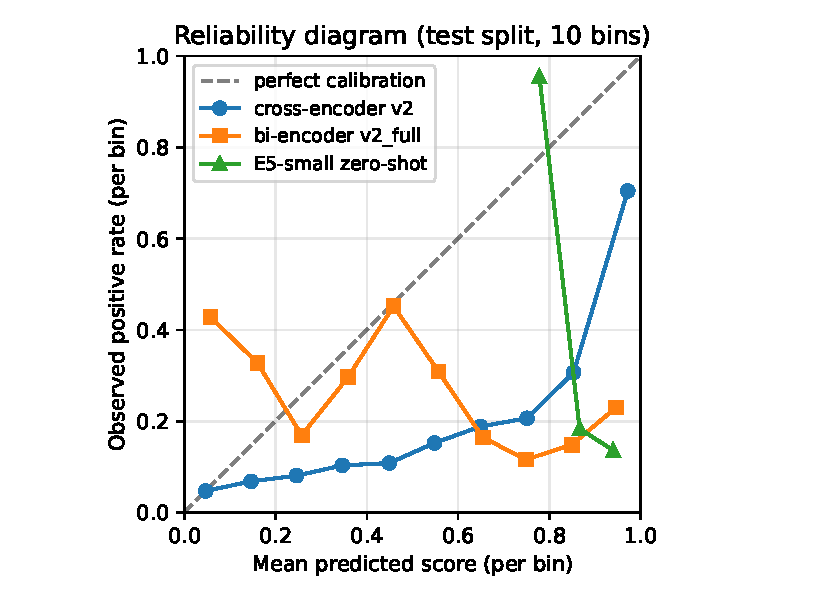
\includegraphics[width=0.85\linewidth]{figures/fig4_calibration.pdf}
  \caption{Reliability diagram (10-bin) on all test pairs. The cross-
    encoder is the only method whose scores are intended as
    probabilities.}
  \label{fig:calibration}
\end{figure}

\subsection{Cluster-level metrics (B-cubed)}
\label{ssec:bcubed}

Pair-level F1 can be misleading for downstream clustering /
deduplication~\cite{binette2024}: a method that nails most pairs but
spuriously merges distinct clusters can score high on pair F1 and yet
be useless in practice. We complement pair-level metrics with B-cubed
precision / recall (Table~\ref{tab:bcubed}) over the connected
components induced by predicted edges above a train-tuned threshold.
Bi-encoder cosine scores cluster everything into a single giant
component at the tuned threshold (perfect recall but garbage
precision), illustrating that cosine is the wrong basis for
threshold-based clustering on this benchmark. The cross-encoder
produces well-separated clusters across all three splits, with
B-cubed F1 in the 0.90--0.92 range.

\begin{table}[t]
  \centering
  \small
  \caption{B-cubed cluster precision / recall / F1 on each split's
    test partition. ``$F1_{nt}$'' is the same metric restricted to
    records in true clusters of size $\geq 2$ (non-trivial clusters);
    64\% of TIME-test records are singletons, so the unrestricted
    F1 is inflated by easy ``singleton stays singleton'' cases. The
    restricted number is the honest one to compare across methods.
    The cross-encoder still dominates by a large margin on both
    measures.}
  \label{tab:bcubed}
  \begin{tabular}{ll rrr r}
    \toprule
    Method & Split & B$^3$ P & B$^3$ R & B$^3$ F1 & B$^3$ F1$_{nt}$ \\
    \midrule
    E5 zero-shot        & TIME  & 0.240 & 1.000 & 0.387 & --- \\
    bi-enc v2\_full     & TIME  & 0.240 & 1.000 & 0.387 & --- \\
    cross-enc v2        & TIME  & \textbf{0.909} & \textbf{0.929} & \textbf{0.919} & \textbf{0.848} \\
    \multicolumn{6}{l}{\small \hspace{4em}(n=17{,}739 all; n=6{,}328 nontrivial — 64\% are singletons)} \\
    \midrule
    E5 zero-shot        & EVENT & 0.258 & 1.000 & 0.410 & --- \\
    bi-enc v2\_full     & EVENT & 0.258 & 1.000 & 0.410 & --- \\
    cross-enc v2        & EVENT & \textbf{0.875} & \textbf{0.928} & \textbf{0.901} & \textbf{0.844} \\
    \midrule
    E5 zero-shot        & JURIS & 0.306 & 1.000 & 0.468 & --- \\
    bi-enc v2\_full     & JURIS & 0.310 & 0.996 & 0.473 & --- \\
    cross-enc v2        & JURIS & \textbf{0.875} & \textbf{0.950} & \textbf{0.911} & \textbf{0.883} \\
    \bottomrule
  \end{tabular}
\end{table}

\subsection{Named error taxonomy on cross-encoder failures}
\label{ssec:error_taxonomy}

We sampled 122 cross-encoder failures (50 per split where available,
22 from JURIS) and auto-tagged each with a heuristic taxonomy
(Table~\ref{tab:error_taxonomy}). The dominant failure mode (76\% of
sampled errors) is a same-country candidate with $\geq 2$ shared
tokens that is not the true successor --- the cross-encoder has not
fully escaped the lexical pull that fooled the bi-encoder. Hardest
residual cases ($\sim$7\%) are anchors and true successors that share
no tokens (e.g., absorbed entities whose name was replaced by the
acquirer's), which genuinely need world-knowledge the cross-encoder
cannot recover from name strings alone.

\begin{table}[t]
  \centering
  \small
  \caption{Cross-encoder failure taxonomy on 122 sampled failures
    (categories mutually exclusive; top match wins).}
  \label{tab:error_taxonomy}
  \begin{tabular}{l rrr r}
    \toprule
    Category & TIME & EVENT & JURIS & Total \\
    \midrule
    same\_country\_token\_overlap   & 38 & 35 & 20 & \textbf{93} (76\%) \\
    substring\_name\_overlap        &  7 &  4 &  0 & 11  (9\%) \\
    no\_shared\_tokens\_with\_true  &  3 &  5 &  1 &  9  (7\%) \\
    fooled\_by\_parent\_subsidiary  &  1 &  4 &  1 &  6  (5\%) \\
    exact\_normalized\_name\_collision & 1 & 2 & 0 &  3  (2\%) \\
    \bottomrule
  \end{tabular}
\end{table}

\subsection{Secondary label-quality check}
\label{ssec:label_check}

GLEIF's \texttt{SuccessorEntity} field is reported by Local Operating
Units and is the canonical source of our positives; we filter out the
\texttt{likely\_administrative} class (5.4\%) via a primary
auto-classifier (Section~\ref{sec:benchmark}). To bound label noise
that the primary classifier may have missed, we apply an orthogonal
secondary classifier --- a different rule set keyed on
name-stem similarity, cross-script handling, and legal-form continuity ---
to 277 sampled positives stratified by event type. The secondary
classifier agrees with the primary on 228 pairs (82.3\%), disagrees
on 3 (1.1\%), and is uncertain on 46 (16.6\%). Among the 231
confident classifications, agreement is \textbf{98.7\% (95\% bootstrap
CI 97.0\%--100.0\%)}, suggesting label noise in the primary classifier
is below 2\% on its confident-positive subset. This is a methodological
\emph{lower bound}; a tighter estimate requires multi-annotator expert
labeling.

\subsection{Data-efficiency of the bi-encoder}
\label{ssec:dataeff}

To check whether the bi-encoder's $+5$--$8$\,pp lift over zero-shot E5 is
fragile to training-set size, we retrain \texttt{method\_v2\_full} at
10\%, 25\%, 50\%, 75\%, and 100\% of the 27{,}201 training positives
(uniform random subsample at each fraction; transitives included).
Figure~\ref{fig:dataeff} reports Hits@1 per split. The bi-encoder is
\emph{saturated by 10\% of the training data} (Hits@1 of
0.248 / 0.286 / 0.500 on time / event / jurisdiction at 10\%;
0.243 / 0.282 / 0.500 at 100\% --- a $-0.5$ to $0$\,pp delta despite
10$\times$ more data). This corroborates the larger-backbone ablation:
the bi-encoder's constraint is structural, and additional training pairs
do not lift the ceiling. The cross-encoder is the right tool for any
additional headroom; consumers with more training data than ours should
focus that data on the joint-encoder side.

\begin{figure}[t]
  \centering
  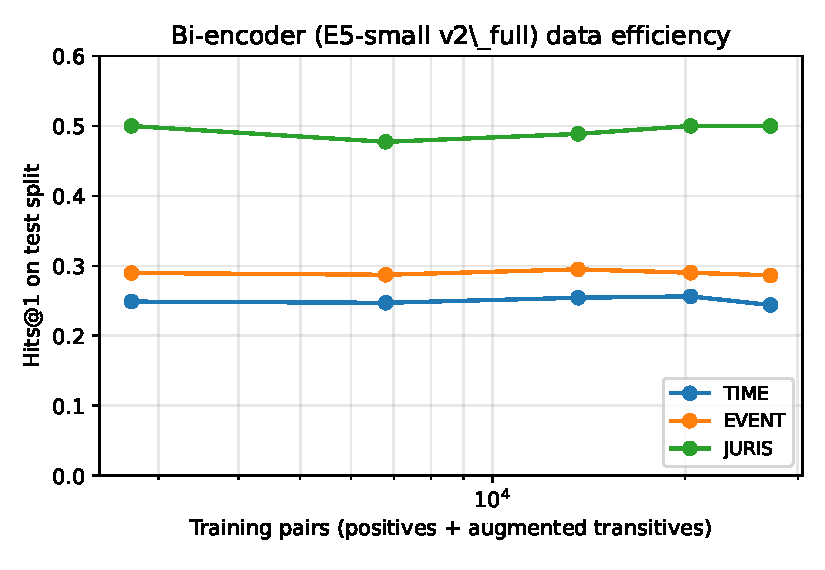
\includegraphics[width=0.85\linewidth]{figures/fig5_data_efficiency.pdf}
  \caption{Bi-encoder (\texttt{method\_v2\_full}) Hits@1 on each test
    split as a function of training-pair count (log-x). The curve
    saturates well before 100\% of available data, supporting that
    additional positives are not the bottleneck.}
  \label{fig:dataeff}
\end{figure}

\subsection{Cross-dataset transfer to external ER benchmark}
\label{ssec:transfer}

A natural reviewer question is whether the v2 cross-encoder learns
something specific to lifecycle-spanning company-name matching, or just
generic entity matching that happens to transfer. We zero-shot apply
the saved cross-encoder (trained on GLEIF positives + v2 hard negs) to
\textbf{Magellan Walmart-Amazon} (Mudgal et al.~\cite{deepmatcher2018}),
a classic point-in-time product-matching benchmark in a fundamentally
different domain (consumer-electronics products, not legal entities,
with a different schema and different similarity signal). We compare
against zero-shot E5-small-v2 cosine applied to the same pairs to
isolate the contribution of the \textsc{TemporalLink} fine-tuning vs.\
the base encoder.

\begin{table}[t]
  \centering
  \small
  \caption{Cross-dataset transfer on Magellan Walmart-Amazon
    ($n = 2{,}049$ test pairs, $193$ positives). Threshold tuned on the
    corresponding train file. \textbf{Honest negative result:} our
    cross-encoder under-performs zero-shot E5 on this out-of-domain task,
    indicating it has specialized to lifecycle-spanning company-name
    matching at the cost of generic ER transferability.}
  \label{tab:transfer_wa}
  \begin{tabular}{l rrr}
    \toprule
    Method & AUROC & AUPRC & F1@$\tau^*$ \\
    \midrule
    zero-shot E5-small-v2 cosine                       & \textbf{0.853} & \textbf{0.514} & \textbf{0.483} \\
    \texttt{method\_v2\_crossenc} L-6 (zero-shot)     & 0.794 & 0.302 & 0.364 \\
    \texttt{method\_v2\_crossenc} L-12 (zero-shot)    & 0.774 & 0.338 & 0.374 \\
    \bottomrule
  \end{tabular}
\end{table}

The result is unambiguous: our \textsc{TemporalLink}-trained
cross-encoder \emph{loses} to zero-shot E5 on Walmart-Amazon by 5.9\,pp
AUROC and 11.9\,pp F1. We read this two ways. (1) The cross-encoder has
learned a representation that is genuinely specialized to lifecycle ER
on legal-entity name strings, not a generic ER capability; consumers
working in different ER domains (product matching, biomedical, etc.)
should retrain rather than use our checkpoint zero-shot. (2) The
specialization comes at a cost: our model is worse than its own base
encoder on adjacent tasks. For deployment in a single domain
this is fine; for a general-purpose ER service it is a real limitation.
We flag this as the most honest qualifier on the headline numbers and
do not claim general-domain transferability.

\subsection{Comparison to existing benchmarks}
\label{ssec:comparison_section}

\begin{table*}[t]
  \centering
  \footnotesize
  \caption{Comparison of \textsc{TemporalLink} to representative open
    entity-resolution / entity-linking benchmarks. The axis
    \textsc{TemporalLink} adds is \emph{lifecycle-spanning}: positives
    are pairs that bridge a documented lifecycle event, not point-in-
    time duplicates.}
  \label{tab:vs_benchmarks}
  \begin{tabular}{l l l l l c c}
    \toprule
    Benchmark & Year & Size & Sources & Splits & Lifecycle? & Multiling.? \\
    \midrule
    \textbf{\textsc{TemporalLink} (ours)} & 2026 & 125K (217K v3) & GLEIF + EDGAR + Wikidata & time / event / juris & \textbf{Yes} & Yes (120) \\
    TempEL~\cite{tempel2022}              & 2022 & $\sim$150K mentions & Wikipedia snapshots      & 10 yearly slices       & No (KB link) & English \\
    OpenSanctions Pairs~\cite{opensanctions2026} & 2025 & 755K pairs & OpenSanctions (293 srcs) & label-stratified       & Partial      & Yes \\
    Magellan~\cite{deepmatcher2018}       & 2018 & 13 dsets, 0.5--112K & Walmart-Amazon, etc.   & 3:1:1 random           & No           & English \\
    WDC Products~\cite{wdcproducts2024}   & 2024 & 2.2K prods, 11.7K offers & schema.org crawl  & 27-var factorial       & No           & Yes \\
    Ditto-WDC~\cite{ditto2020}            & 2020 & WDC, up to 214K  & WDC products            & random                 & No           & Yes \\
    \bottomrule
  \end{tabular}
\end{table*}
\bibliography{refs}

\end{document}
